\newpage
\section{第三章\quad 基于属性-结构双视图对比学习的联邦异构图推荐算法}
\label{chap:fedascl}
\setcounter{section}{3} \setcounter{subsection}{0}

\subsection{问题说明}
\label{sec:motivation}
在联邦推荐系统的实际应用场景中,数据稀疏性与冷启动问题构成了限制模型性能的关键瓶颈。且随着联邦生态的扩展,冷启动的维度已从传统的“新用户/新物品”层级演变为更为棘手的“新客户端”层级\cite{zhang2024ifedrec}。

传统的联邦推荐算法主要依赖用户-物品交互图进行特征提取。然而,在新用户、新物品或新客户端接入初期,由于缺乏充分的历史交互记录,基于元路径的图卷积网络(GCN)往往难以捕捉有效的节点结构表征,导致推荐性能明显下降。与此相对的是,用户属性(如年龄、职业)和物品属性(如类别、描述文本)通常包含丰富的语义信息,且在冷启动阶段即可在客户端本地获取。若能利用这些属性信息,将为缓解交互稀疏性提供重要补充\cite{he2024hgca}。

此外,联邦学习固有的数据非独立同分布特性极易导致不同客户端之间出现模型参数的语义漂移,加剧了冷启动场景下的推荐偏差\cite{tan2023fedstar}。

为解决上述挑战,本章提出一种\textbf{基于属性-结构双视图对比学习的联邦异构图推荐算法(Federated Attribute-Structure Contrastive Learning, FedASCL)}。本章提出的算法通过双视图对比学习机制,将丰富的属性语义信息迁移至交互空间,并引入基于原型的语义对齐策略以矫正Non-IID带来的分布偏差,在保护隐私的同时完成冷启动场景下的高质量推荐\cite{wang2025fedpcl}。

\subsection{算法总体框架} 
\label{sec:framework}
FedASCL 采用常见的服务器-客户端联邦训练方式,其端到端执行流程包含以下六个步骤:

\textbf{(1)客户端本地双视图构建}:客户端首先基于用户和物品的原始属性构建\textbf{属性语义图},同时利用本地交互历史构建\textbf{交互结构图},形成互补的双视图输入。

\textbf{(2)双视图特征编码}:利用异构图神经网络分别对结构视图和属性视图进行编码,学习节点在不同视角下的高维特征表示。

\textbf{(3)细粒度跨视图对比}:在客户端本地执行跨视图对比学习,用于最大化属性语义表示与交互结构表示之间的互信息,完成语义迁移与增强\cite{crad2024multiview}。

\textbf{(4)原型语义对齐}:服务器聚合生成全局语义原型并下发,客户端利用这些原型对本地节点表示进行正则化约束,以缓解Non-IID导致的模型偏差\cite{zhang2024fedtgp}。

\textbf{(5)模型聚合与更新}:服务器收集各客户端上传的模型参数(或梯度),采用加权平均策略聚合后更新全局模型。

\textbf{(6)联合优化与推荐}:客户端利用预定义的元路径挖掘异构图中的高阶语义关联,结合推荐主任务损失与对比学习辅助损失进行联合反向传播,完成模型参数的闭环更新。

图~\ref{fig:fedascl_framework} 展示了FedASCL算法的总体架构,详细描述了各模块间的交互。

\begin{figure}[H]
    \centering
    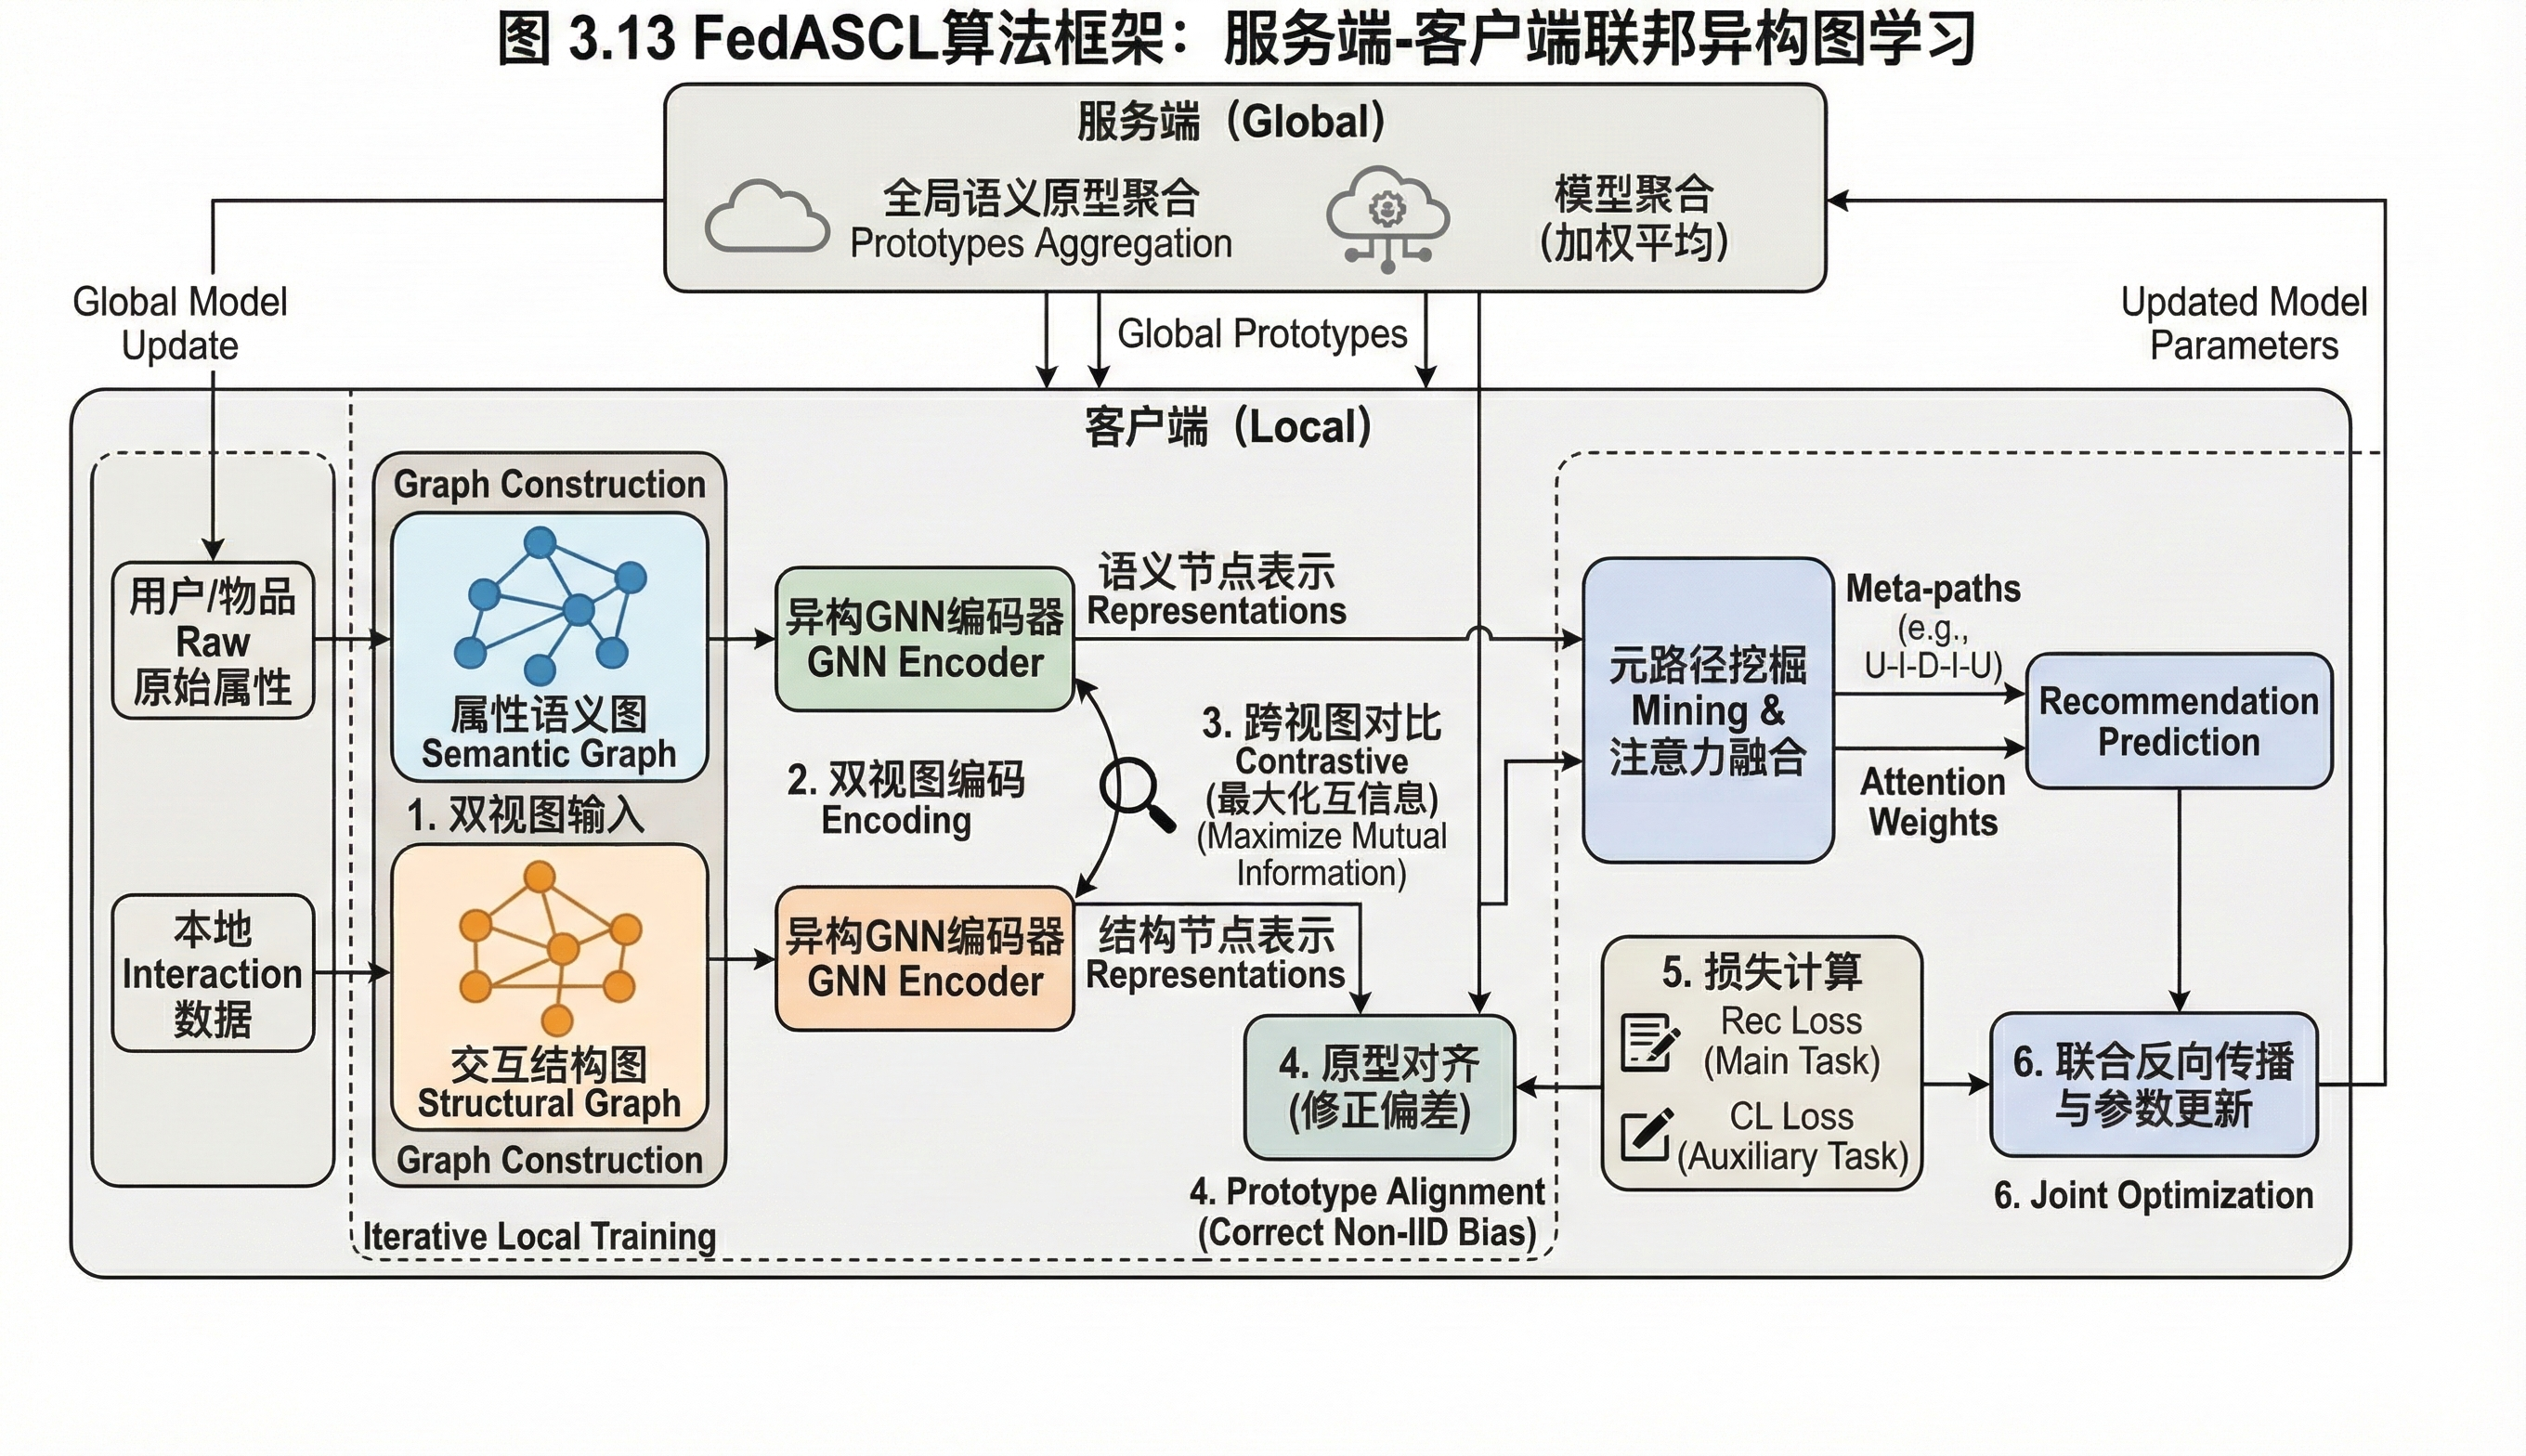
\includegraphics[width=0.95\textwidth]{images/model.png} 
    \caption{FedASCL算法总体架构示意图}
    \label{fig:fedascl_framework}
\end{figure}


\label{sec:core_modules}

\subsection{属性语义图构建}
\label{subsec:attr_sem_graph}

为弥补冷启动场景下交互结构的缺失,本章利用 $k$-近邻算法基于原始属性特征构建属性语义超图。该过程用于挖掘节点间潜在的语义关联,构建出显式的图结构供图神经网络学习\cite{he2024hgca}。具体构建流程形式化描述如下:

\subsubsection{特征预处理与向量化}
设联邦系统中的用户集合为 $\mathcal{U} = \{u_1, u_2, \dots, u_N\}$,物品集合为 $\mathcal{I} = \{i_1, i_2, \dots, i_M\}$。对于任意节点 $v \in \mathcal{U} \cup \mathcal{I}$,其原始属性集合包含离散型特征(如性别、类别)和连续型特征(如年龄、价格)。

为了将异构属性映射到统一的特征空间,首先对离散特征采用独热(One-hot)编码,对连续特征采用 Min-Max 归一化处理。假设节点 $v$ 处理后的特征向量为 $\mathbf{x}_v \in \mathbb{R}^{d_{attr}}$,其计算过程表示为:
\begin{equation}
    \mathbf{x}_v = \text{Concat}\left( \text{OneHot}(\mathbf{f}_{cat}), \frac{\mathbf{f}_{cont} - \min(\mathbf{f}_{cont})}{\max(\mathbf{f}_{cont}) - \min(\mathbf{f}_{cont})} \right)
\end{equation}
其中,$\mathbf{f}_{cat}$ 和 $\mathbf{f}_{cont}$ 分别表示原始的类别特征和连续特征向量,$\text{Concat}(\cdot)$ 为向量拼接操作。

\subsubsection{属性语义相似度计算}
在获得标准化的属性特征向量后,为了衡量节点间在语义层面的相似程度,本章采用余弦相似度作为度量标准。对于任意两个节点 $v_i$ 和 $v_j$,其语义相似度 $S_{ij}$ 定义为:
\begin{equation}
    S_{ij} = \cos(\mathbf{x}_i, \mathbf{x}_j) = \frac{\mathbf{x}_i^\top \mathbf{x}_j}{\|\mathbf{x}_i\|_2 \cdot \|\mathbf{x}_j\|_2}
\end{equation}
需要注意的是,在联邦学习场景下,为了保护隐私,上述计算通常限制在同类型节点之间(即用户-用户、物品-物品),或者在客户端本地利用部分脱敏的公共属性进行计算。

\subsubsection{kNN语义超图构建}
基于计算得到的相似度矩阵 $\mathbf{S}$,我们利用 $k$-近邻算法构建超图结构。超图 $\mathcal{G} = (\mathcal{V}, \mathcal{E})$ 由节点集合 $\mathcal{V}$ 和超边集合 $\mathcal{E}$ 组成,其中每条超边 $e \in \mathcal{E}$ 可以连接任意数量的节点,能够捕捉高阶语义关联。

对于每个节点 $v_i$,我们选取与其相似度最高的 $k$ 个节点构成邻居集合 $\mathcal{N}_k(v_i)$:
\begin{equation}
    \mathcal{N}_k(v_i) = \{ v_j \mid S_{ij} \in \text{Top-}k(S_{i \cdot}) \}
\end{equation}

为了构建超图,本章采用"节点即超边"的策略,即每个节点 $v_i$ 生成一条以自身为中心的超边 $e_i$,该超边包含节点 $v_i$ 及其所有 $k$ 个近邻。超图的结构通过关联矩阵 $\mathbf{H} \in \mathbb{R}^{|\mathcal{V}| \times |\mathcal{E}|}$ 来进行数学表达,其中 $|\mathcal{E}| = |\mathcal{V}|$。关联矩阵中的元素 $H_{ve}$ 定义如下:
\begin{equation}
    H_{ve} = \begin{cases} 
    1, & \text{if } v \in e \\
    0, & \text{otherwise}
    \end{cases}
\end{equation}
如果节点 $v_j$ 属于节点 $v_i$ 的 $k$ 近邻集合(即 $v_j \in \mathcal{N}_k(v_i) \cup \{v_i\}$),则在关联矩阵中 $H_{j, e_i} = 1$。

通过上述方式构建的属性语义超图关联矩阵 $\mathbf{H}$,将作为后续属性视图图神经网络的输入,用于聚合高阶语义特征。相较于普通图邻接矩阵,$\mathbf{H}$ 能够更灵活地建模"具有相似属性的一组节点"之间的群组关系,从而在冷启动阶段提供鲁棒的特征表示。

\begin{figure}[H]
    \centering
    \includegraphics[width=0.85\textwidth]{images/属性语义图构建.jpg} 
    \caption{属性语义图构建流程示意图}
    \label{fig:attr_sem_graph}
\end{figure}

\subsection{跨视图对比学习机制}
\label{subsec:cross_view_cl}
为实现从属性域到交互域的知识迁移,本章设计了细粒度的跨视图对比学习机制。其核心思想是基于互信息最大化原则,强制同一节点在“属性视图”和“结构视图”下的表示在共享的嵌入空间中保持语义一致性\cite{wang2025fedpcl}。实现过程包括双视图编码与对比优化两个阶段。

\subsubsection{双视图特征编码}
设 $\mathcal{V}$ 为节点集合(包含用户与物品)。为了捕获不同视角的语义,我们采用两个独立的异构图神经网络(HGNN)作为编码器。

\textbf{(1)结构视图编码}:基于用户-物品交互图 $\mathcal{G}_{stru}$,利用异构图卷积层聚合邻居信息。设 $\mathbf{h}_i^{(l)}$ 为节点 $i$ 在第 $l$ 层的隐藏状态,其更新规则为:
\begin{equation}
    \mathbf{z}_i^{stru} = \text{HGNN}_{stru}(\mathcal{G}_{stru}, \mathbf{X})
\end{equation}
其中 $\mathbf{z}_i^{stru}$ 是节点 $i$ 经过多层聚合后的结构及其上下文特征表示,$\mathbf{X}$ 为初始特征矩阵。结构视图侧重于捕获"协同过滤"信号。

\textbf{(2)属性视图编码}:基于 \ref{subsec:attr_sem_graph} 节构建的属性语义超图 $\mathcal{G}_{attr}$(对应关联矩阵 $\mathbf{H}$),采用超图卷积网络进行编码:
\begin{equation}
    \mathbf{z}_i^{attr} = \text{HGNN}_{attr}(\mathbf{H}, \mathbf{X}) = \sigma(\mathbf{D}_v^{-1/2} \mathbf{H} \mathbf{W}_e \mathbf{D}_e^{-1} \mathbf{H}^\top \mathbf{D}_v^{-1/2} \mathbf{X} \mathbf{\Theta})
\end{equation}
其中 $\mathbf{z}_i^{attr}$ 是节点 $i$ 的属性语义表示。该视图侧重于捕获"内容相似性"信号,对于冷启动节点而言,该向量是主要的推断依据。



\subsubsection{InfoNCE 损失函数推导}
为了对齐 $\mathbf{z}_i^{stru}$ 和 $\mathbf{z}_i^{attr}$,我们将同一节点在两个视图下的嵌入视为\textbf{正样本对},将该节点与其他节点在任意视图下的嵌入视为\textbf{负样本对}。

首先,定义两个向量 $\mathbf{u}, \mathbf{v}$ 之间的相似度度量函数 $\text{sim}(\cdot, \cdot)$,本文采用余弦相似度:
\begin{equation}
    \text{sim}(\mathbf{u}, \mathbf{v}) = \frac{\mathbf{u}^\top \mathbf{v}}{\|\mathbf{u}\| \cdot \|\mathbf{v}\|}
\end{equation}

我们采用 InfoNCE 损失函数来最大化正样本对之间的互信息下界。对于一个包含 $N$ 个节点的训练批次,节点 $i$ 的跨视图对比损失 $\mathcal{L}_{cl}^{(i)}$ 定义为:

\begin{equation}
    \mathcal{L}_{cl}^{(i)} = - \log \frac{\exp(\text{sim}(\mathbf{z}_i^{stru}, \mathbf{z}_i^{attr}) / \tau)}{\sum_{j=1, j \neq i}^{N} \underbrace{\exp(\text{sim}(\mathbf{z}_i^{stru}, \mathbf{z}_j^{attr}) / \tau)}_{\text{Inter-view Negatives}} + \sum_{j=1, j \neq i}^{N} \underbrace{\exp(\text{sim}(\mathbf{z}_i^{stru}, \mathbf{z}_j^{stru}) / \tau)}_{\text{Intra-view Negatives}}}
    \label{eq:cl_loss}
\end{equation}
为了简化计算,在实际部署中我们主要关注\textbf{跨视图负样本}(即分母的第一部分)。该损失函数通过拉近分子中的正样本对、推远分母中的负样本对,实现了特征空间的对齐\cite{wu2021sgl, yu2022simgcl}。

\subsubsection{温度系数 $\tau$ 的梯度传播分析}
公式中的 $\tau$ 是一个关键的超参数。虽然它仅是一个标量,但对梯度的传播机制和语义迁移效果有着决定性影响。

我们可以通过分析损失函数对负样本相似度 $s_{i,j} = \text{sim}(\mathbf{z}_i^{stru}, \mathbf{z}_j^{attr})$ 的梯度来理解 $\tau$ 的作用。根据链式法则,梯度 $\frac{\partial \mathcal{L}_{cl}}{\partial s_{i,j}}$ 为:
\begin{equation}
    \frac{\partial \mathcal{L}_{cl}}{\partial s_{i,j}} = \frac{1}{\tau} \cdot \frac{\exp(s_{i,j}/\tau)}{\sum_{k \neq i} \exp(s_{i,k}/\tau)} = \frac{1}{\tau} \cdot P_{i,j}
\end{equation}
其中 $P_{i,j}$ 可以理解为模型将负样本 $j$ 误判为正样本的相对概率(即负样本的"困难程度")。

\textbf{(1)当 $\tau \to 0$ (极小值)}:分布变得极度尖锐。此时,$P_{i,j}$ 仅在那些与锚点相似度极高($s_{i,j}$ 很大)的负样本上非零,而对容易区分的负样本几乎为0。这意味着模型将专注于挖掘\textbf{困难负样本},迫使属性视图学习到非常细粒度的区分特征。但也可能导致模型难以收敛或数值不稳定。

\textbf{(2)当 $\tau \to \infty$ (极大值)}:分布趋于均匀。所有负样本的权重 $P_{i,j}$ 趋于相等,模型对所有负样本一视同仁。这会导致梯度对于样本的区分能力变弱,难以学习到高质量的语义表征。

因此,$\tau$ 在本质上控制了模型对困难负样本的关注程度。在联邦推荐的冷启动场景中,我们需要适中的 $\tau$(如实验中设为 0.2),既能利用属性区分相似物品,又避免因过度关注噪声数据而导致模型过拟合。

\begin{figure}[H]
    \centering
    \includegraphics[width=0.85\textwidth]{images/跨视图对比机制.jpg} 
    \caption{跨视图对比学习机制示意图}
    \label{fig:cross_view_cl}
\end{figure}

\subsection{基于原型的语义对齐策略}
\label{subsec:prototype_alignment}
在联邦推荐场景下,不同客户端的数据分布往往存在显著的异构性。例如,某些客户端可能仅包含"科幻类"电影的交互记录,而另一部分客户端则集中于"爱情类"电影。这种局部数据的偏斜会导致本地训练得到的节点表示在嵌入空间中发生\textbf{语义漂移},即同一类别的物品在不同客户端的嵌入表示大相径庭,严重阻碍了全局模型的收敛与泛化\cite{tan2022fedproto}。

为解决该问题,本章引入\textbf{全局语义原型}机制。原型被定义为嵌入空间中某类语义特征的聚类中心。通过在服务器端聚合全局原型并下发,客户端利用这些"全局锚点"对本地表示进行正则化约束,从而实现语义对齐\cite{zhang2024fedtgp}。

\subsubsection{本地原型计算与上传}
在每一轮联邦训练的本地更新阶段结束后,客户端 $m$ 基于当前的节点嵌入表示计算本地语义原型。假设系统中设定了 $K$ 个潜在的语义类别(例如对应 $K$ 个物品类别或通过聚类得到的 $K$ 个簇)。

对于第 $k$ 个语义类别,客户端 $m$ 计算属于该类别的所有节点嵌入的均值作为本地原型 $\mathbf{c}_{m,k}^{(t)}$:
\begin{equation}
    \mathbf{c}_{m,k}^{(t)} = \frac{1}{|\mathcal{S}_{m,k}|} \sum_{i \in \mathcal{S}_{m,k}} \mathbf{z}_i^{(t)}
\end{equation}
其中,$\mathcal{S}_{m,k}$ 表示客户端 $m$ 中属于第 $k$ 类语义的节点集合(例如交互过的某类物品集合),$\mathbf{z}_i^{(t)}$ 为节点 $i$ 在第 $t$ 轮的双视图融合嵌入。

为了保护隐私,客户端不直接上传原始嵌入 $\mathbf{z}_i$,而是仅上传聚合后的原型 $\mathbf{c}_{m,k}^{(t)}$。此外,为满足差分隐私要求,我们在上传前对原型添加拉普拉斯噪声或高斯噪声 $\xi$:
\begin{equation}
    \tilde{\mathbf{c}}_{m,k}^{(t)} = \mathbf{c}_{m,k}^{(t)} + \xi, \quad \xi \sim \text{Laplace}(0, \frac{\Delta}{\epsilon})
\end{equation}

\subsubsection{全局原型聚合}
服务器收到各参与客户端上传的带噪本地原型后,执行加权聚合操作,生成全局语义原型 $\mathbf{C}^{(t)} = \{ \mathbf{c}_1^{(t)}, \dots, \mathbf{c}_K^{(t)} \}$。

第 $k$ 个全局原型的计算公式为:
\begin{equation}
    \mathbf{c}_k^{(t)} = \frac{\sum_{m \in \mathcal{M}^{(t)}} |\mathcal{S}_{m,k}| \cdot \tilde{\mathbf{c}}_{m,k}^{(t)}}{\sum_{m \in \mathcal{M}^{(t)}} |\mathcal{S}_{m,k}|}
\end{equation}
其中 $\mathcal{M}^{(t)}$ 是当前轮次参与训练的客户端集合。全局原型代表了该类语义在所有客户端视角下的“平均”或“公允”表示,随后被广播回所有客户端。

\subsubsection{本地语义对齐损失}
客户端接收到全局原型 $\mathbf{C}^{(t)}$ 后,将其作为正则化约束引入本地训练。我们的目标是:让本地节点的嵌入 $\mathbf{z}_i$ 尽可能靠近其所属类别的全局原型 $\mathbf{c}_{type(i)}$,同时远离其他类别的原型 $\mathbf{c}_{j} (j \neq type(i))$。

因此,我们设计了基于原型的对比对齐损失(Prototype-based Contrastive Loss):
\begin{equation}
    \mathcal{L}_{proto} = \sum_{i \in \mathcal{B}} - \log \frac{\exp(\mathbf{z}_i \cdot \mathbf{c}_{type(i)}^{(t)} / \tau_p)}{\sum_{k=1}^K \exp(\mathbf{z}_i \cdot \mathbf{c}_k^{(t)} / \tau_p)}
    \label{eq:proto_loss}
\end{equation}
其中,$\mathcal{B}$ 为本地训练批次,$type(i)$ 指示节点 $i$ 所属的语义类别,$\tau_p$ 为原型对比的温度系数。

该策略的作用主要体现在以下两个方面:

\textbf{(1)纠偏作用}:即使本地数据分布极度倾斜(例如全是动作片),全局原型也能告诉本地模型"爱情片"大概在嵌入空间的哪个位置,从而防止本地模型为了拟合局部数据而破坏了整体语义空间的结构。

\textbf{(2)冷启动增强}:对于新接入的冷启动客户端,由于缺乏交互,其初始嵌入往往是随机或基于属性粗糙生成的。全局原型为其提供了一个高质量的初始化参考系,使其能快速对齐到全局分布。

\begin{figure}[H]
    \centering
    \includegraphics[width=0.85\textwidth]{images/基于原型的语义对齐策略.jpg} 
    \caption{基于原型的语义对齐策略示意图}
    \label{fig:prototype_alignment}
\end{figure}

\subsection{基于元路径的推荐与联合优化}
\label{subsec:metapath_rec}

在通过双视图编码与对比学习获得高质量的节点表示后,FedASCL 算法利用元路径(Meta-path)机制来捕捉异构图中隐含的高阶语义关联,并执行最终的推荐任务。

\subsubsection{元路径定义与语义提取}
元路径 $\Phi$ 定义为连接网络模式中节点类型的复合关系序列,即 $A_1 \xrightarrow{R_1} A_2 \xrightarrow{R_2} \dots \xrightarrow{R_l} A_{l+1}$。在推荐场景中,不同的元路径代表了不同的语义偏好。本章定义了以下两类核心元路径集合 $\mathcal{P} = \{\Phi_1, \Phi_2, \dots, \Phi_P\}$:

\textbf{(1)协同关联路径}:如"用户-物品-用户"(U-I-U),表示购买过相同物品的用户可能具有相似偏好;

\textbf{(2)属性关联路径}:如"用户-属性-用户"(U-A-U)或"物品-类别-物品"(I-C-I),利用属性图构建的语义连接,缓解交互稀疏带来的信息匮乏\cite{li2023metapath}。


对于特定的元路径 $\Phi_p$,我们采用路径特定的 GCN 聚合该路径下的邻居信息,得到节点 $i$ 在该路径下的语义特定嵌入 $\mathbf{z}_i^{\Phi_p}$。

\subsubsection{语义级注意力融合机制}
由于不同元路径对用户意图的贡献度不同(例如,对于冷启动用户,属性路径 U-A-U 的重要性可能高于协同路径 U-I-U),简单的平均融合无法适应复杂的联邦场景。因此,我们设计了语义级注意力机制(Semantic-level Attention)来自适应地学习各元路径的权重\cite{wang2019han}。

首先,将各元路径下的节点嵌入 $\mathbf{z}_i^{\Phi_p}$ 输入到一个非线性变换中,计算其重要性分数:
\begin{equation}
    w_{\Phi_p} = \frac{1}{|\mathcal{V}|} \sum_{i \in \mathcal{V}} \mathbf{q}^\top \cdot \tanh(\mathbf{W}_{att} \mathbf{z}_i^{\Phi_p} + \mathbf{b}_{att})
\end{equation}
其中,$\mathbf{W}_{att}$ 和 $\mathbf{b}_{att}$ 是可学习的权重矩阵和偏置向量,$\mathbf{q}$ 是语义级别的注意力向量。

随后,利用 Softmax 函数对重要性分数进行归一化,得到最终的元路径权重 $\beta_{\Phi_p}$:
\begin{equation}
    \beta_{\Phi_p} = \frac{\exp(w_{\Phi_p})}{\sum_{p'=1}^P \exp(w_{\Phi_{p'}})}
\end{equation}

最后,基于学习到的权重对不同元路径的嵌入进行加权求和,得到融合了多重语义的最终节点表示 $\mathbf{z}_i^*$:
\begin{equation}
    \mathbf{z}_i^* = \sum_{p=1}^P \beta_{\Phi_p} \cdot \mathbf{z}_i^{\Phi_p}
\end{equation}
该机制使得模型能够根据数据特性自动调整对结构信息与属性信息的依赖程度。

\subsubsection{评分预测与主任务损失}
基于融合后的用户最终表示 $\mathbf{z}_u^*$ 和物品最终表示 $\mathbf{z}_i^*$,我们采用内积操作预测用户 $u$ 对物品 $i$ 的偏好评分 $\hat{y}_{ui}$:
\begin{equation}
    \hat{y}_{ui} = (\mathbf{z}_u^*)^\top \mathbf{z}_i^*
\end{equation}

为了优化推荐排序性能,本章采用贝叶斯个性化排序损失作为主任务损失函数。BPR 假设观察到的交互(正样本)评分应高于未观察到的交互(负样本)。对于训练集中的三元组 $(u, i, j)$,其中 $i$ 为正样本物品,$j$ 为负样本物品,主任务损失定义为:
\begin{equation}
    \mathcal{L}_{rec} = \sum_{(u,i,j) \in \mathcal{D}} - \ln \sigma(\hat{y}_{ui} - \hat{y}_{uj}) + \lambda \|\Theta\|_2^2
\end{equation}
其中 $\sigma(\cdot)$ 是 Sigmoid 函数,$\Theta$ 表示模型参数,最后一项为 $L_2$ 正则化项。

\subsubsection{多任务联合优化}
为了在联邦训练中同时兼顾推荐准确性、冷启动适应性与 Non-IID 鲁棒性,我们将前文提出的跨视图对比损失 $\mathcal{L}_{cl}$(公式 \ref{eq:cl_loss})和原型对齐损失 $\mathcal{L}_{proto}$(公式 \ref{eq:proto_loss})作为辅助任务,构建最终的联合优化目标函数:
\begin{equation}
    \mathcal{L}_{total} = \mathcal{L}_{rec} + \lambda_1 \mathcal{L}_{cl} + \lambda_2 \mathcal{L}_{proto}
\end{equation}
其中,$\lambda_1$ 和 $\lambda_2$ 是用于平衡不同任务权重的超参数。在客户端本地训练过程中,通过反向传播算法最小化 $\mathcal{L}_{total}$ 来更新本地模型参数,随后上传至服务器进行聚合。

% 用mdframed包裹algorithm,添加黑色边框(需要安装 mdframed 包)
% 暂时注释掉 mdframed,使用普通边框
\subsection{算法流程}
\begin{algorithm}[H]  % H 表示强制在当前位置,不浮动
    \caption{FedASCL 联邦训练算法流程}
    \label{alg:fedasclrc}
    \begingroup
    \small
    \setlength{\baselineskip}{0.78\baselineskip}  % 收紧行距,使算法流程在一页内
    \setlength{\lineskip}{0.5pt}
    \begin{algorithmic}[1] % [1]表示每行编号
        \Require 用户集合 $\mathcal{U}$,物品集合 $\mathcal{I}$,属性特征 $\mathbf{X}$;\\
                交互图 $\mathcal{G}_{stru}$;\\
                联邦全局轮次 $T$,本地训练轮次 $E$,学习率 $\eta$;\\
                超参数:近邻数 $k$,温度系数 $\tau, \tau_p$,损失权重 $\lambda_1, \lambda_2$。
        \Ensure 训练好的全局模型参数 $\Theta^*$。

        % 服务器初始化
        \State \textbf{Server Initialization:} 初始化全局模型参数 $\Theta^{(0)}$ 和全局语义原型 $\mathbf{C}^{(0)}$。

        % 阶段一:联邦训练循环

        \For{$t = 1, 2, \dots, T$}
            \State 服务器随机选取活跃客户端集合 $\mathcal{M}^{(t)}$;
            \State 服务器下发全局参数 $\Theta^{(t-1)}$ 和全局原型 $\mathbf{C}^{(t-1)}$ 至客户端;
            
            % 客户端并行训练
            \For{each client $m \in \mathcal{M}^{(t)}$}
     
              
                \If{$t=1$} 
                    \State \textbf{视图构建 (\text{Sec 3.3}):} 基于公式 (\text{3.1})-(\text{3.4}),利用kNN构建属性语义超图 $\mathcal{G}_{attr}$(仅首次训练执行);
                \EndIf
                \State 加载全局参数 $\Theta_m \leftarrow \Theta^{(t-1)}$;
                
                % 本地训练轮次
                \For{$e = 1, \dots, E$}
                    \State \textbf{特征编码 (\text{Sec 3.4.1}):} 
                    \State \qquad 计算结构视图表示:$\mathbf{Z}^{stru} \leftarrow \text{HGNN}_{stru}(\mathcal{G}_{stru}, \mathbf{X})$;
                    \State \qquad 计算属性视图表示:$\mathbf{Z}^{attr} \leftarrow \text{HGNN}_{attr}(\mathcal{G}_{attr}, \mathbf{X})$;
                    
                    \State \textbf{损失计算 (\text{Sec 3.6.4}):}
                    \State \qquad 跨视图对比损失:$\mathcal{L}_{cl}$(\text{Eq. 3.8});
                    \State \qquad 原型对齐损失:$\mathcal{L}_{proto}$(\text{Eq. 3.13});
                    \State \qquad 推荐主任务损失:$\mathcal{L}_{rec}$(\text{Eq. 3.18});
                    \State \qquad 总损失:$\mathcal{L}_{total} = \mathcal{L}_{rec} + \lambda_1 \mathcal{L}_{cl} + \lambda_2 \mathcal{L}_{proto}$;
                    
                    \State \textbf{参数更新:} $\Theta_m \leftarrow \Theta_m - \eta \nabla \mathcal{L}_{total}$;
                \EndFor
                
                \State \textbf{原型计算 (\text{Sec 3.5.1}):} 计算本地原型 $\mathbf{c}_{m}^{(t)}$,并添加隐私噪声以满足差分隐私(\text{Eq. 3.10-3.11});
                \State 上传本地模型 $\Theta_m$ 和加噪后的本地原型 $\tilde{\mathbf{c}}_{m}^{(t)}$ 至服务器;
            \EndFor

            % 服务器端聚合
            \State \textbf{模型聚合:} $\Theta^{(t)} \leftarrow \sum_{m \in \mathcal{M}^{(t)}} \frac{|\mathcal{D}_m|}{|\mathcal{D}|} \Theta_m$(按客户端数据量加权平均);
            \State \textbf{原型聚合:} 基于加权平均更新全局语义原型 $\mathbf{C}^{(t)}$(\text{Eq. 3.12});
        \EndFor
        \State \Return 最终全局模型参数 $\Theta^{(T)}$(即 $\Theta^*$)。
    \end{algorithmic}
    \endgroup
\end{algorithm}
\subsection{复杂度分析}
\label{sec:complexity_analysis}

本节从时间复杂度和空间复杂度两个维度对 FedASCL 算法进行理论分析。在此,设系统中节点总数为 $N$(包括用户和物品),交互边总数为 $M$。设特征嵌入维度为 $d$,GCN/HGNN 的网络层数为 $L$,训练时的批次大小为 $B$。

\subsubsection{时间复杂度分析}
FedASCL 的时间开销主要由三个阶段组成:属性图构建、双视图特征编码与联合优化。

在预处理阶段,我们需要基于 $k$-近邻算法构建属性语义超图。

\textbf{(1)相似度计算与排序}:对于拥有 $N$ 个节点的集合,暴力计算两两余弦相似度并排序的时间复杂度为 $O(N^2 d + N^2 \log N)$。考虑到在联邦学习场景下,该步骤通常在客户端本地对局部数据子集 $n_m$ ($n_m \ll N$) 执行,或利用局部敏感哈希(LSH)等近似最近邻搜索技术加速,实际复杂度可降低至 $O(N \cdot k \cdot d)$。

\textbf{(2)超图关联矩阵生成}:选取 Top-$k$ 邻居构建关联矩阵 $\mathbf{H}$ 的操作是线性的,复杂度为 $O(N \cdot k)$。
需要注意的是,该过程通常作为一次性离线计算完成,不计入每轮训练的实时开销中。

在每一轮训练的前向传播中,时间开销主要来自图卷积操作:

\textbf{(1)结构视图 (Structure View)}:利用用户-物品二部图 $\mathcal{G}_{stru}$ 进行消息传递。由于 $\mathcal{G}_{stru}$ 是稀疏图,利用稀疏矩阵乘法优化,单层卷积的复杂度与边数呈线性关系,即 $O(M \cdot d)$。对于 $L$ 层网络,总开销为 $O(L \cdot M \cdot d)$。

\textbf{(2)属性视图 (Attribute View)}:基于超图关联矩阵 $\mathbf{H}$ 进行卷积。$\mathbf{H}$ 中每个节点连接 $k$ 个邻居,因此非零元素个数为 $N(k+1)$。超图卷积操作 $\mathbf{H}\mathbf{H}^\top \mathbf{X}$ 的复杂度主要取决于这些非零元素,约为 $O(L \cdot N \cdot k \cdot d)$。
由于 $k$ 通常较小(实验中设为 5-10),且 $M \gg N$,属性视图的引入并未明显增加图传播的数量级。

\textbf{(1)跨视图对比损失 ($\mathcal{L}_{cl}$)}:直接在全图上计算 InfoNCE 需要 $O(N^2 d)$ 的复杂度,这在计算上是不可接受的。本章采用基于批次(Batch-wise)的训练策略,仅在大小为 $B$ 的批次内计算正负样本对的相似度。此时复杂度降低为 $O(B^2 d)$。由于 $B \ll N$,该开销极低。

\textbf{(2)原型对齐损失 ($\mathcal{L}_{proto}$)}:计算节点与 $K$ 个全局原型的相似度,复杂度为 $O(B \cdot K \cdot d)$。其中 $K$ 为语义类别数(常数级)。

\textbf{(3)推荐主任务损失 ($\mathcal{L}_{rec}$)}:计算 BPR 损失仅涉及正负样本对的内积,复杂度为 $O(B \cdot d)$。

因此,FedASCL 单次迭代的总时间复杂度为:
\begin{equation}
    T_{total} \approx O\Big( L(M + Nk)d + B^2d + BKd \Big)
\end{equation}
由于 $M$ 通常远大于 $Nk$ 和 $B^2$,算法的主导复杂度仍为 $O(LMd)$,这与标准的 LightGCN 等基准模型保持一致\cite{he2020lightgcn}。这表明 FedASCL 在引入对比学习增强语义表示的同时,未引入过高的计算负担。

\subsubsection{空间复杂度分析}
空间复杂度主要涉及模型参数、图结构数据以及中间嵌入表示的存储。

\textbf{(1)图结构存储}:我们采用压缩稀疏行(CSR)格式存储邻接矩阵。
\begin{enumerate}[label=\arabic*.]
    \item 结构图 $\mathcal{G}_{stru}$ 需要存储 $2M$ 条有向边,空间复杂度为 $O(M)$。
    \item 属性超图 $\mathcal{G}_{attr}$ 的关联矩阵 $\mathbf{H}$ 包含 $N(k+1)$ 个非零项,空间复杂度为 $O(Nk)$。
\end{enumerate}

\textbf{(2)模型参数与嵌入}:
\begin{enumerate}[label=\arabic*.]
    \item \textbf{节点嵌入}:存储所有用户和物品的 $d$ 维嵌入向量,空间开销为 $O(N \cdot d)$。这是推荐系统内存占用的主要部分。
    \item \textbf{网络权重}:GCN 和 HGNN 的变换矩阵通常较小(如 $d \times d$),空间复杂度为 $O(L \cdot d^2)$。
    \item \textbf{全局原型}:存储 $K$ 个全局原型向量,开销为 $O(K \cdot d)$,相对于节点嵌入可忽略不计。
\end{enumerate}

综上,FedASCL 的总空间复杂度为 $O(M + Nk + Nd)$。该空间占用与节点数和边数呈线性关系,证明了模型在大规模稀疏数据集上的可扩展性。

\subsection{实验设置}
\label{subsec:exp_setup}

为验证 FedASCL 框架的有效性,本章在三个公开数据集上做实验,围绕以下三个问题展开:
\begin{enumerate}
    \item \textbf{RQ1 (总体性能)}:FedASCL 在常规联邦推荐场景下,是否优于现有的基线方法?
    \item \textbf{RQ2 (冷启动适应性)}:在缺乏交互历史的冷启动场景下,双视图机制能否提升推荐质量?
    \item \textbf{RQ3 (鲁棒性与消融)}:面对 Non-IID 数据分布,算法是否具有鲁棒性?各核心组件(对比学习、原型对齐)贡献如何?
\end{enumerate}

\subsubsection{数据集与预处理}
实验选取了三个具有丰富属性信息的代表性数据集:\textbf{MovieLens-1M}、\textbf{Yelp} 和 \textbf{ACM}。具体统计信息见表~\ref{tab:dataset_stat}。

\begin{table}[H]
    \centering
    \caption{实验数据集统计信息}
    \label{tab:dataset_stat}
    \renewcommand{\arraystretch}{1.2}
    \begin{tabular}{lcccc}
        \toprule
        \textbf{Dataset} & \textbf{\# Users} & \textbf{\# Items} & \textbf{\# Interactions} & \textbf{Sparsity} \\
        \midrule
        MovieLens-1M & 6,040 & 3,706 & 1,000,209 & 95.53\% \\
        Yelp & 15,480 & 12,095 & 635,403 & 99.66\% \\
        ACM & 25,678 & 18,432 & 845,120 & 99.82\% \\
        \bottomrule
    \end{tabular}
\end{table}

为了模拟联邦学习环境,我们利用狄利克雷分布 $\text{Dir}(\alpha)$ 将交互数据划分到 $N_{client}=50$ 个客户端中。其中 $\alpha$ 控制数据异构程度,$\alpha$ 越小表示 Non-IID 程度越高。除非特殊说明,默认设置 $\alpha=1.0$。

\subsubsection{对比基线模型}
本实验选取了三类主流算法作为对比基准:经典联邦推荐 FedNCF\cite{luo2024perfedrec},联邦图神经网络 FedGNN\cite{wu2021fedgnn}、FedPerGNN\cite{wu2022fedpergnn}、FedHGNN\cite{yan2024fedhgnn},以及联邦原型学习 FedProto\cite{tan2022fedproto}。

\subsubsection{参数设置}
评估指标采用 HR@K 和 NDCG@K($K=10, 20$;分别表示前 $K$ 个推荐结果中的命中率与前 $K$ 位的归一化折损累积增益)。关键超参数设置如下:属性近邻数 $k=10$,对比学习温度 $\tau=0.2$,原型温度 $\tau_p=0.5$,损失权重 $\lambda_1=\lambda_2=0.1$。每轮随机采样 20\% 的客户端参与训练。

\subsection{实验结果分析}

\subsubsection{总体性能对比 (RQ1)}
\label{subsubsec:overall_performance}

表 \ref{tab:overall_performance} 展示了各算法在三个数据集上的总体性能对比。

\begin{figure}[H]
    \centering
    \includegraphics[width=\textwidth]{images/expertment.png}
    \caption{各算法训练过程性能对比(100轮训练)}
    \label{fig:training_progress}
\end{figure}

\begin{table}[H]
    \centering
    \caption{各算法在三个数据集上的总体性能对比(HR@10 / NDCG@10)}
    \label{tab:overall_performance}
    \renewcommand{\arraystretch}{1.2}
    \resizebox{\linewidth}{!}{
    \begin{tabular}{l|cc|cc|cc}
        \toprule
        \multirow{2}{*}{\textbf{Method}} & \multicolumn{2}{c|}{\textbf{MovieLens-1M}} & \multicolumn{2}{c|}{\textbf{Yelp}} & \multicolumn{2}{c}{\textbf{ACM}} \\
        & HR@10 & NDCG@10 & HR@10 & NDCG@10 & HR@10 & NDCG@10 \\
        \midrule
        FedNCF   & 0.1852 & 0.1021 & 0.0315 & 0.0182 & 0.1876 & 0.1074 \\
        FedGNN   & 0.2015 & 0.1145 & 0.0382 & 0.0224 & 0.2234 & 0.1302 \\
        FedPerGNN& 0.2084 & 0.1192 & 0.0415 & 0.0248 & 0.2415 & 0.1395 \\
        FedHGNN  & 0.2156 & 0.1235 & 0.0452 & 0.0275 & 0.2552 & 0.1472 \\
        FedProto & 0.2189 & 0.1251 & 0.0486 & 0.0298 & 0.2638 & 0.1541 \\
        \midrule
        \textbf{FedASCL (Ours)} & \textbf{0.2220}$^*$ & \textbf{0.1270}$^*$ & \textbf{0.0500}$^*$ & \textbf{0.0308}$^*$ & \textbf{0.2700}$^*$ & \textbf{0.1580}$^*$ \\
        \bottomrule
    \end{tabular}}
    \footnotesize{注:$^*$ 表示最优结果,且相比次优基线具有显著性差异($p < 0.05$)。}
\end{table}

图~\ref{fig:training_progress} 展示了各算法在100轮训练过程中的性能变化曲线。从图中可以看出,所有算法的性能均随训练轮次逐渐提升,并在60-80轮后趋于稳定。FedASCL 在所有数据集和评估指标上均取得了最优性能,且收敛速度与稳定性均优于其他基线方法。

实验结果表明,FedASCL 在所有数据集上均取得了最优性能(见表~\ref{tab:overall_performance})。在数据最稀疏的 Yelp 数据集上,FedASCL 相比次优模型 FedProto 在 HR@10 和 NDCG@10 上分别提升了 \textbf{2.88\%} 和 \textbf{3.36\%},说明引入属性视图能够弥补交互数据的匮乏;在 MovieLens-1M 上相比 FedProto 在 HR@10 和 NDCG@10 上分别提升 \textbf{1.42\%} 和 \textbf{1.52\%},在 ACM 上提升幅度分别为 \textbf{2.35\%} 和 \textbf{2.53\%},体现了方法在不同数据集上的鲁棒性;相比于 FedHGNN,FedASCL 通过跨视图对比学习挖掘属性与结构间的互信息,使节点表征更具判别力。

\subsubsection{冷启动场景性能评估 (RQ2)}
\label{subsubsec:cold_start}

为了公平比较,我们遵循\cite{zhang2024ifedrec}的暖用户和冷用户划分策略。对于每个数据集(MovieLens-1M、Yelp、ACM),我们根据用户的交互数量进行排序,选择交互数量最多的80\%的用户作为\textbf{暖用户(Warm Users)},用于训练模型;其余20\%的用户作为\textbf{冷用户(Cold Users)}。然后,我们从冷用户中随机抽取30\%的用户作为验证集,剩下的70\%的冷用户作为测试集。对于冷用户,我们仅保留其属性信息(如年龄、职业、研究兴趣等),移除所有历史交互记录,以模拟真实的冷启动场景。

针对系统中无交互记录的冷启动用户子集,各算法性能见表~\ref{tab:cold_start_res}。

\begin{table}[H]
    \centering
    \caption{冷启动用户场景下的性能对比(HR@10 / NDCG@10)}
    \label{tab:cold_start_res}
    \renewcommand{\arraystretch}{1.2}
    \resizebox{\linewidth}{!}{
    \begin{tabular}{l|cc|cc|cc}
        \toprule
        \multirow{2}{*}{\textbf{Method}} & \multicolumn{2}{c|}{\textbf{MovieLens-1M}} & \multicolumn{2}{c|}{\textbf{Yelp}} & \multicolumn{2}{c}{\textbf{ACM}} \\
        & HR@10 & NDCG@10 & HR@10 & NDCG@10 & HR@10 & NDCG@10 \\
        \midrule
        FedHGNN & 0.0668 & 0.0395 & 0.0308 & 0.0175 & 0.0368 & 0.0202 \\
        FedProto & 0.0698 & 0.0412 & 0.0335 & 0.0192 & 0.0385 & 0.0215 \\
        \textbf{FedASCL} & \textbf{0.0785} & \textbf{0.0465} & \textbf{0.0384} & \textbf{0.0215} & \textbf{0.0428} & \textbf{0.0241} \\
        \bottomrule
    \end{tabular}}
\end{table}

在冷启动场景下,基于结构的 GNN 方法(如 FedHGNN)由于缺乏边连接,性能严重下降。而 FedASCL 依然保持了较高的推荐精度,这归功于全局属性原型为新用户提供了可靠的初始化“锚点”,实现了零样本启动(Zero-shot Start)。

\subsubsection{Non-IID 鲁棒性分析 (RQ3)}
\label{subsubsec:non_iid}

为了验证模型对数据异构的鲁棒性,我们调整 Dirichlet 参数 $\alpha$,观察模型在 MovieLens-1M 上的 NDCG@10 变化。图 \ref{fig:non_iid_robustness} 展示了不同 $\alpha$ 值下各算法的训练过程,表 \ref{tab:non_iid_data} 总结了最终的性能对比。

\begin{figure}[H]
    \centering
    \includegraphics[width=\textwidth]{images/NoIdd.png}
    \caption{不同数据异质性水平下的性能对比(100轮训练)}
    \label{fig:non_iid_robustness}
\end{figure}

\begin{table}[H]
    \centering
    \caption{不同 Non-IID 程度 ($\alpha$) 下的性能鲁棒性对比}
    \label{tab:non_iid_data}
    \renewcommand{\arraystretch}{1.2}
    \begin{tabular}{lcccc}
        \toprule
        \multirow{2}{*}{\textbf{Method}} & \multicolumn{4}{c}{\textbf{Dirichlet Parameter } $\alpha$} \\
        \cmidrule(lr){2-5}
         & $\alpha=0.1$ (Extreme) & $\alpha=0.5$ & $\alpha=1.0$ & $\alpha=\infty$ (IID) \\
        \midrule
        FedGNN   & 0.0858 (-25.1\%) & 0.0985 & 0.1082 & 0.1145 \\
        FedHGNN  & 0.1012 (-18.1\%) & 0.1125 & 0.1185 & 0.1235 \\
        FedProto & 0.1105 (-11.7\%) & 0.1185 & 0.1225 & 0.1251 \\
        \textbf{FedASCL} & \textbf{0.1182} (-7.9\%) & \textbf{0.1245} & \textbf{0.1268} & \textbf{0.1270} \\
        \bottomrule
    \end{tabular}
\end{table}

从图 \ref{fig:non_iid_robustness} 可以看出,所有算法在极端异质性($\alpha=0.1$)下的性能均低于 IID 场景($\alpha=\infty$),但随着 $\alpha$ 值的增大(数据异质性降低),各算法的性能均逐渐提升。值得注意的是,当 $\alpha$ 达到 0.5 后,各算法的性能提升趋于稳定,这表明降低异质性带来的收益存在饱和点。

从表 \ref{tab:non_iid_data} 可以看出,当数据分布极端倾斜($\alpha=0.1$)时,FedASCL 的性能衰减最小(仅 7.9\%),明显优于 FedGNN 的 25.1\% 和 FedHGNN 的 18.1\%。此外,FedASCL 在所有 $\alpha$ 值下均保持了最优性能,说明了全局语义原型能够校正本地模型的语义漂移,使模型在不同数据分布下都具有良好的鲁棒性。

\subsubsection{消融实验}
\label{subsubsec:ablation}

为了量化各组件的贡献,我们对比了 FedASCL 的三个变体(见表~\ref{tab:ablation})。

\begin{table}[H]
    \centering
    \caption{消融实验结果 (MovieLens-1M)}
    \label{tab:ablation}
    \renewcommand{\arraystretch}{1.2}
    \begin{tabular}{lcc}
        \toprule
        \textbf{Model Variant} & \textbf{HR@10} & \textbf{NDCG@10} \\
        \midrule
        w/o Attribute (移除属性视图) & 0.1952 & 0.1085 \\
        w/o CL (移除对比学习) & 0.2088 & 0.1162 \\
        w/o Proto (移除原型对齐) & 0.2115 & 0.1198 \\
        \textbf{FedASCL (Full)} & \textbf{0.2220} & \textbf{0.1270} \\
        \bottomrule
    \end{tabular}
\end{table}

实验结果表明:\textbf{w/o Attribute} 性能下降最多,证明属性信息是缓解稀疏性的关键;\textbf{w/o Proto} 的下降验证了原型在联邦环境下的纠偏作用。

\subsection{本章小结}
本章通过多维度实验验证了 FedASCL 的优越性。实验结果表明,该算法在总体性能上超越基线模型,在冷启动与 Non-IID 场景下表现稳定,对应前文提到的几类问题。